% ------------------------------------------------------------------------------%%%%%%%%
\section{Theory - \textit{clDice} in Digital Topology}
\label{sec:interp}


In addition to our Theorem 1 in the main paper, %\ref{thm2},
we are providing intuitive interpretations of \textit{clDice} from the digital topology perspective. Betti numbers describe and quantify topological differences in algebraic topology. The first three Betti numbers ($\beta_0$, $\beta_1$, and $\beta_2$) comprehensively capture the manifolds appearing in 2D and 3D topological space. Specifically,
\begin{itemize}[itemsep=-4pt]%leftmargin=*]
    \item $\beta_0$ represents the number of \textit{connected-components},
    \item $\beta_1$ represents the number of \textit{circular holes}%[c.f. Fig. A. \ref{fig_top_ex}]
    , and
    \item $\beta_2$ represents the number of \textit{cavities} %[c.f. Fig. A. \ref{fig_top_ex}] 
    (Only in 3D)
\end{itemize}{}


\begin{figure}[ht!]
\begin{center}

\includegraphics[width=0.13\textwidth]{figs/hole_2d.pdf}
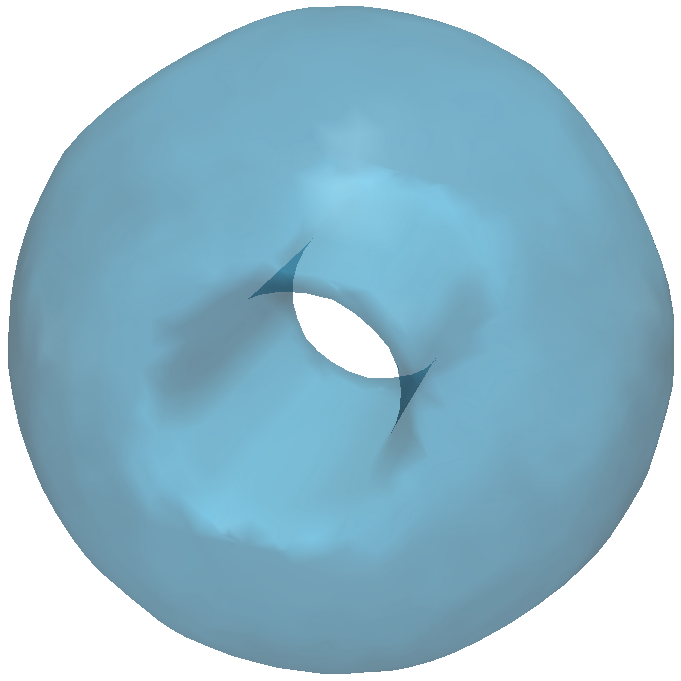
\includegraphics[width=0.14\textwidth]{figs/hole.png}
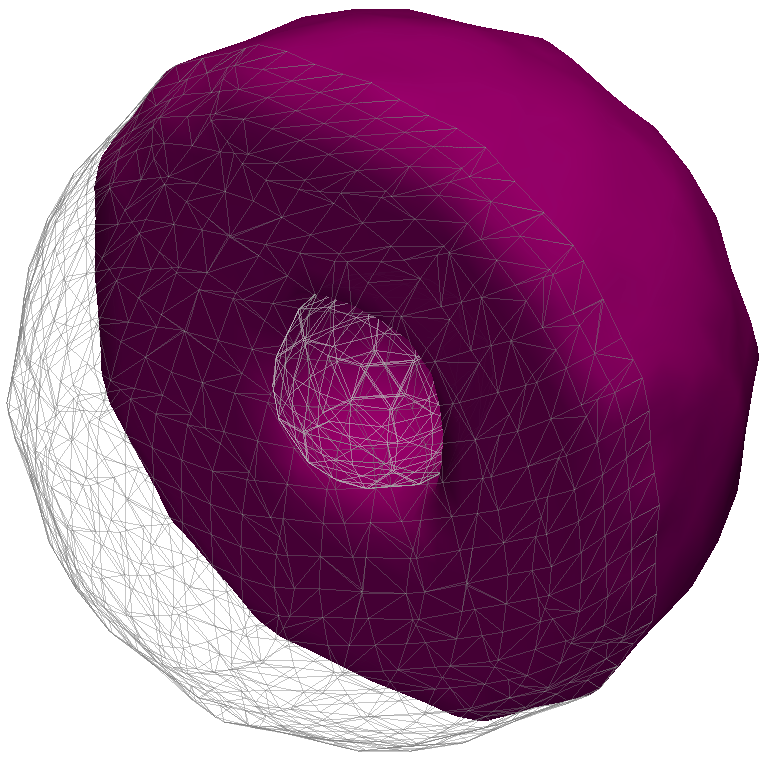
\includegraphics[width=0.14\textwidth]{figs/cavity.png} \\
\end{center}
\caption{Examples of the topology properties. Left, a hole in 2D, in the middle a hole in 3D and right a cavity inside a sphere in 3D.} 
\label{fig_top_ex}
\end{figure}

Using the concepts of Betti numbers and digital topology by Kong et al. \cite{kong1995topology,rosenfeld1979digital}, we formulate the effect of topological changes between a true binary mask ($V_L$) and a predicted binary mask ($V_P$) in Fig. \ref{fig_ghost_miss}. We will use the following definition of \textbf{ghosts} and \textbf{misses}, see Figure \ref{fig_ghost_miss}.


\begin{enumerate}[] %label=\textbf{Top \arabic*},align=left
    \item \textbf{Ghosts in skeleton: } We define ghosts in the predicted skeleton ($S_P$) when $S_P \not\subset V_L$. This means the predicted skeleton is not completely included in the true mask. In other words, there exist false-positives in the prediction, which survive after skeletonization.\label{prop1}
    
    \item \textbf{Misses in skeleton: } We define misses in the predicted skeleton ($S_P$) when $S_L \not\subset V_P$. This means the true skeleton is not completely included in the predicted mask. In other words, there are false-negatives in the prediction, which survive after skeletonization.\label{prop2}
\end{enumerate}



\begin{figure*}[ht!]
\begin{center}

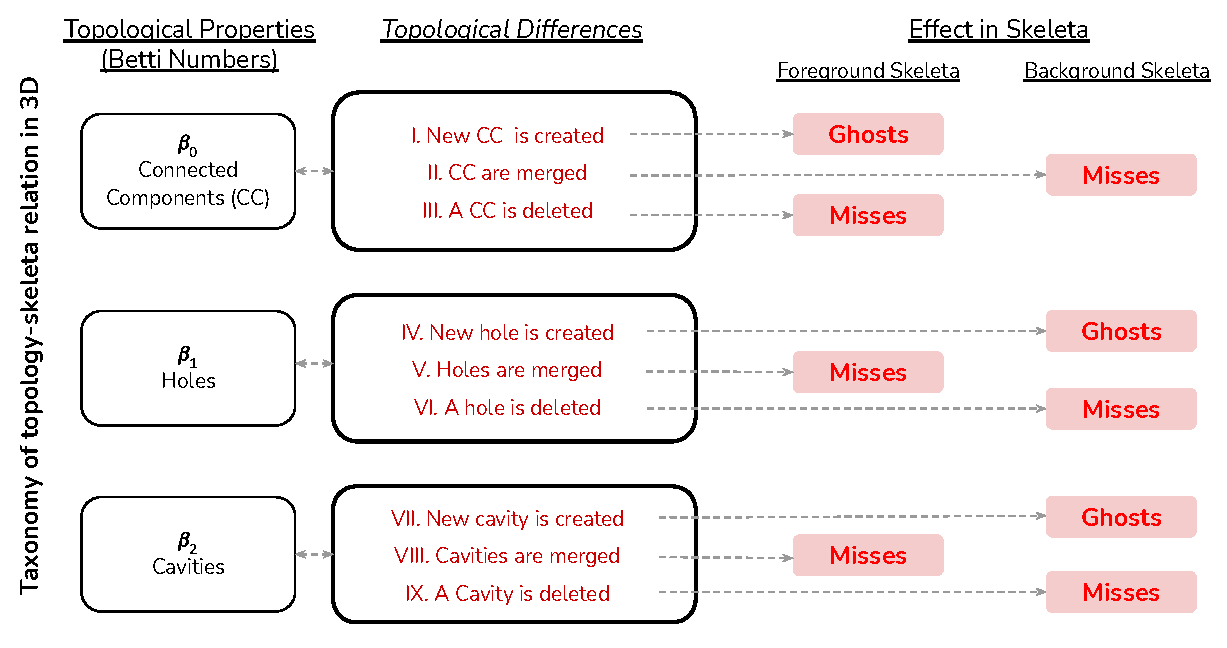
\includegraphics[width=0.95\linewidth]{figs/clDice_CVPR.pdf}
\label{fig_theory}
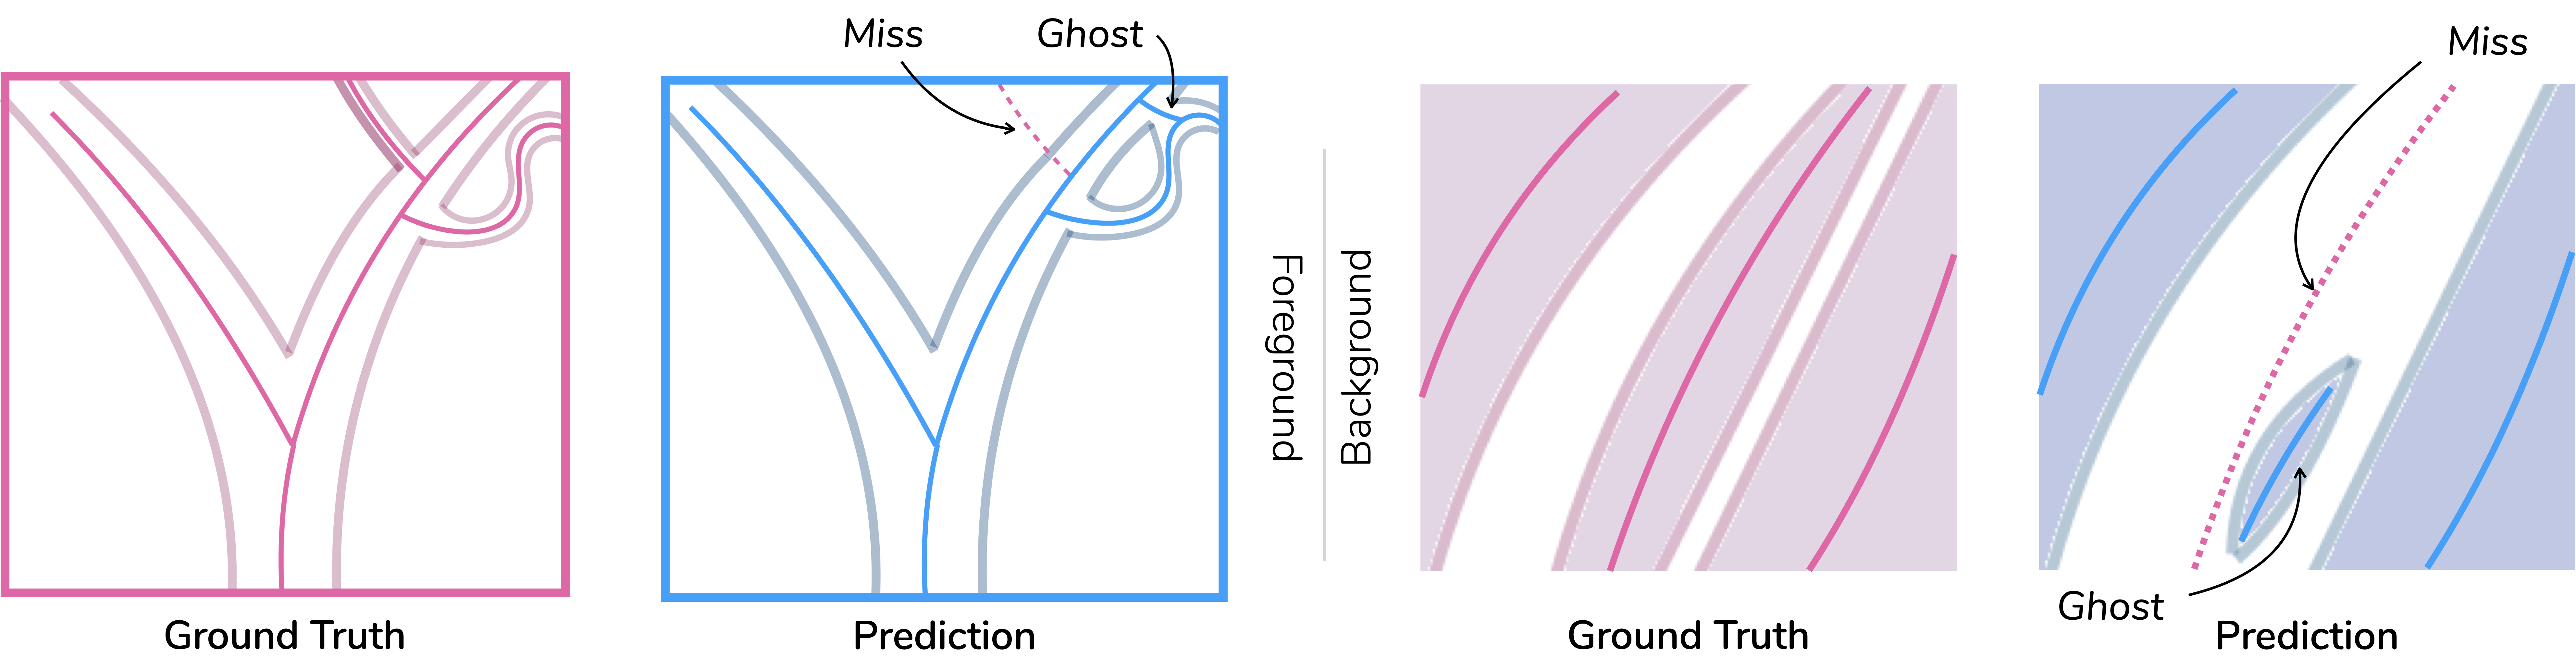
\includegraphics[width=0.92\linewidth]{figs/ghost_miss_cvpr.png}
\end{center}
\caption{Upper part, left, taxonomy of the $iff$ conditions to preserve topology in 3D using the concept of Betti numbers \cite{kong1995topology,kong1989digital}; interpreted as the necessary violation of skeleton properties for any possible topological change in the terminology of ghosts and misses (upper part right) . Lower part, intuitive depictions of ghosts and misses in the prediction; for the skeleton of the foreground (left) and the skeleton of the background (right).}
\label{fig_ghost_miss}
\end{figure*}

The false positives and false negatives are denoted by $V_P\setminus V_L$ and $V_L\setminus V_P$, respectively, where $\setminus$ denotes a set difference operation. The loss function aims to minimize both errors. We call an error correction to happen when the value of a previously false-negative or false-positive voxel flips to a correct value. Commonly used voxel-wise loss functions, such as Dice-loss, treat every false-positive and false-negative equally, irrespective of the improvement in regards to topological differences upon their individual error correction. Thus, they cannot guarantee homotopy equivalence until and unless every single voxel is correctly classified. In stark contrast, we show in the following proposition that \textit{clDice} guarantees homotopy equivalence under \textit{a minimum error correction.}


% \noindent 
\begin{proposition}

For any topological differences between $V_P$ and $V_L$, achieving optimal \textit{clDice} to guarantee homotopy equivalence requires a minimum error correction of $V_P$.
\end{proposition}

\begin{proof}
From Fig \ref{fig_ghost_miss}, any topological differences between $V_P$ and $V_L$ will result in ghosts or misses in the foreground or background skeleton. Therefore, removing ghosts and misses are sufficient conditions to remove topological differences. Without the loss of generalizability, we consider the case of ghosts and misses separately:\\

For a \textbf{ghost} $g \subset S_P, \exists \mbox{ a set of predicted voxels } E1 \subset \{V_P \setminus V_L\}\mbox{ such that } V_P \setminus E
1$ does not create any misses and removes $g$. Without the loss of generalizability, let's assume that there is only one ghost $g$. Now, to remove $g$, under a minimum error correction of $V_P$, we have to minimize $|E1|$. Let's say an optimum solution $E1_{min}$ exists. By construction, this implies that $V_P\setminus E1_{min}$ removes $g$.


For a \textbf{miss} $m \subset V_P^\complement, \exists \mbox{ a set of predicted voxels } E2 \subset \{V_L \setminus V_P\}\mbox{ such that } V_P \cup E2$ does not create any ghosts and removes $m$. Without the loss of generalizability, let's assume that there is only one miss $m$. Now, to remove $m$, under a minimum error correction of $V_P$, we have to minimize $|E2|$. Let's say an optimum solution $E2_{min}$ exists. By construction, this implies that $V_P\cup E2_{min}$ removes $m$.\\

Thus, in the absence of any ghosts and misses, from Lemma \ref{obs1}, \textit{clDice}=1 for both foreground and background. Finally, Therefore, Theorem 1 (from the main paper) guarantees homotopy equivalence.
\end{proof}


\begin{restatable}[]{lemma}{obsone}
\label{obs1}
In the absence of any ghosts and misses \textit{clDice}=1.
\end{restatable}

\begin{proof}
The absence of any ghosts $S_P \in V_L$ implies $Tprec=1$; and the absence of any misses $S_L \in V_P$ implies $Tsens=1$. Hence, \textit{clDice}=1.
\end{proof}